\documentclass{article}
\usepackage{amsmath}
\usepackage{amssymb}
\usepackage{esvect}
\usepackage[usenames, dvipsnames]{color}
\usepackage{fancyhdr}
\usepackage{hyperref}
\usepackage{pgfplots}
\usepackage{tikz}
\usepackage{geometry}
\usepackage[normalem]{ulem}

\geometry{letterpaper, portrait, margin=0.5in}
\pagestyle{fancy}

\fancyhf{} % clear all header fields
\renewcommand{\headrulewidth}{0pt}
\fancyfoot[LE,RO]{\thepage}           % page number in "outer" position of footer line
\fancyfoot[RE,LO]{\copyright\;aquarc 2025. \href{https://aquarc.org}{\underline{aquarc.org}}} % other info in "inner" position of footer line

\definecolor{myred1}{RGB}{255, 0, 0}
\definecolor{myyellow1}{RGB}{255, 255, 219}
\definecolor{mygreen1}{RGB}{0, 255, 0}
\definecolor{mygreen2}{RGB}{0, 126, 0}
\definecolor{myblue1}{RGB}{0, 0, 255}

\begin{document}

\fontsize{14}{16}\selectfont

% center the title
\begin{center}
    \textbf{\underline{Min/Max and Point of Inflection Cheatsheet}}
\end{center}

\tableofcontents
\pagebreak


\section{Min/Max}

To check for a minimum or maximum, you set $f'(x)=0$ to obtain the \textbf{critical points}. Not all of them are going to be maxima or minima, and sometimes neither. 

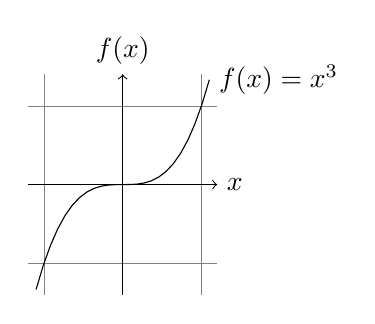
\begin{tikzpicture}[domain=-1.1:1.1]
    \draw[very thin,color=gray] (-1.2,-1.4) grid (1.2,1.4);
    \draw[->] (-1.2,0) -- (1.2,0) node[right] {$x$};
    \draw[->] (0,-1.4) -- (0,1.4) node[above] {$f(x)$};
    \draw plot (\x,\x^3) node[right] {$f(x) =x^3$};
\end{tikzpicture}

\begin{enumerate}
    \item If $f''(x)<0$ and $f'(x)=0$, then $(x,f(x))$ is a maximum 
    \item If $f''(x)>0$ and $f'(x)=0$, then $(x,f(x))$ is a minimum
    \item If $f''(x)=0$ and $f'(x)=0$, then $(x,f(x))$ is indeterminate; check if signs change or use a Taylor approximation instead (not practical). 
\end{enumerate}

\subsection{Taylor Approximation}

A Taylor Series is used to approximate a point $x$ from $f(x)$ using a series around $c$. It looks like:

\begin{align}
    \sum_{n=0}^{\infty}{\frac{f^{(n)}(c)}{n!}(x-c)^n}
\end{align}

Because no sole derivative will give you enough information from the function at one point (illustrated by $f(x)=x^3$, $x^4$, $x^5$...) you need to know all the derivatives. And if the function isn't smooth (differentiable for each $x$ where $x \in \mathbb{R}$, this method can't be used analytically either.

\section{Point of Inflection}

Points of Inflection \textbf{may} exist when $f''(x)=0$ or are undefined. You have to use Taylor approximations to figure out if it actually is a point of inflection. It is preferable to check if the signs change.

\subsection{Examples}

These problems are taken from \textit{Calculus for the AP Course} by Michael Sullivan. 

\begin{enumerate}
    \item The function $f$ has a second derivative given by $f''(x)=x^2(x-1)\sqrt{x+1}$. At what values of $x$ does $f(x)$ have a point of inflection?

    At a quick glance, potential points of inflection are $x=-1,0,1$. However, we need to plug in values between each of these potential inflection points to find where $f''(x)$ switches from negative to positive or vice versa. You can also figure out that $x^2$ and $\sqrt{x+1}$ will always return a positive value, so the only solution is $x=1$.

    \item Let $g$ be the function given by $g(x)=\int_0^{x^2}{e^{-t^2}}dt$. The function $g$ has a point of inflection at $x=$

    Let $f(x)=e^{-x^2}$. Let $F(x)$ represent its antiderivative.

    \begin{align*}
        g(x)=F(x^2)-F(0) \\
        g'(x)=2xF'(x^2) \\
        \Longrightarrow g'(x)=2xe^{-x^4} \\
        g''(x)=2e^{-x^4}+2xe^{-x^4}*(-4x^3) \\
        0=2e^{-x^4}(1-4x^4) \\
        x^4=\frac{1}{4}
        x=\pm \frac{\sqrt{2}}{2}
    \end{align*}

    It is good practice to test that these inflection points are actually inflection points, but if you are short on time you can just pick the MCQ that includes eiither or both $\pm\frac{\sqrt{2}}{2}$.

\end{enumerate}

\end{document}
